% !Mode:: "TeX:UTF-8:Main"
% gif command (hope it still works ...)
% magick -density 160 -delay 35 -loop 0 XXXX.pdf XXXX.gif
% this here slower, around 105!
% magick -density 160 -delay 100 -loop 0 XXXX.pdf XXXX.gif

% delay 105 => 100/105 FPS
% Needed: 25 FPS
% => increase number of pages by 25/(100/105) = 26.25
% => show each page 26 times

\PassOptionsToPackage{svgnames,x11names}{xcolor}
\documentclass{beamer}
\usepackage[T1]{fontenc} % or fontspec if lualatex is wanted ...
\setbeamertemplate{navigation symbols}{}
\usepackage{tikzlings-marmots}
\setbeamertemplate{background}{}
\setbeamertemplate{background canvas}{}
\newcommand\openclose{close}
\begin{document}
\begin{frame}
\begin{tikzpicture}[remember picture,overlay]
% Background image
\node[at=(current page.center)]{%
	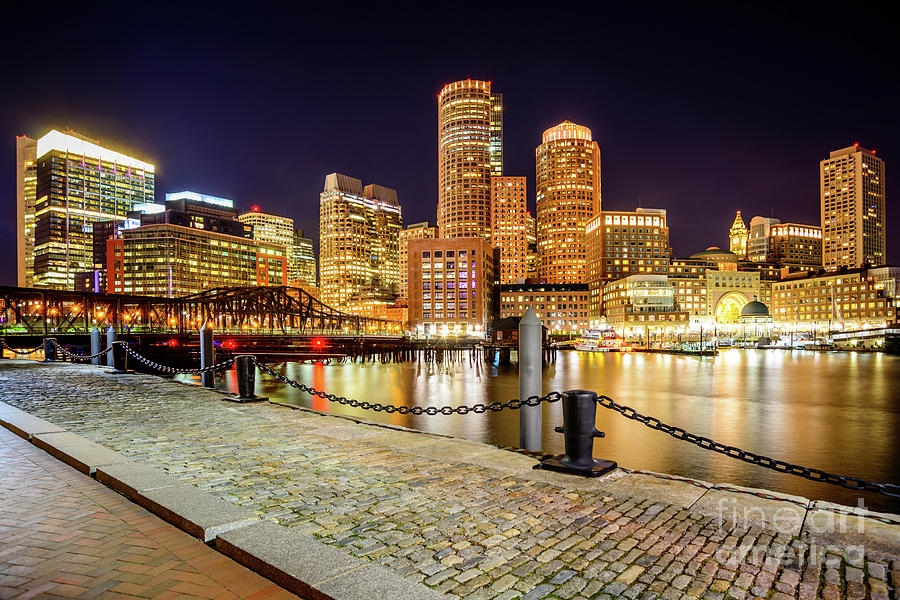
\includegraphics[height=\paperheight]{boston-skyline}
};	
	

% Image credit of background
\node[at=(current page.south),yshift=0.25cm,text width=\paperwidth,font=\tiny,align=center,white]{%
	\url{https://images.fineartamerica.com/images/artworkimages/mediumlarge/1/boston-skyline-at-night-and-harborwalk-picture-paul-velgos.jpg}
};
\end{tikzpicture}

\foreach\x in {1,2,...,25}{%
  \ifodd\x \renewcommand\openclose{close}\else\renewcommand\openclose{open}\fi
  \only<\x>{%
  \vspace*{2cm}
  \includegraphics[scale=0.8]{marmot-\openclose}
\includegraphics[scale=0.85,trim=0cm 0.75cm 0cm 0cm]{marmot-\openclose}
\includegraphics[scale=0.9,trim=0cm 1.5cm 0cm 0cm]{marmot-\openclose}
\includegraphics[scale=0.95,trim=0cm 2.25cm 0cm 0cm]{marmot-\openclose}}}


\end{frame}

\begin{frame}
\begin{tikzpicture}[remember picture,overlay]
% Background image
\node[at=(current page.center)]{%
	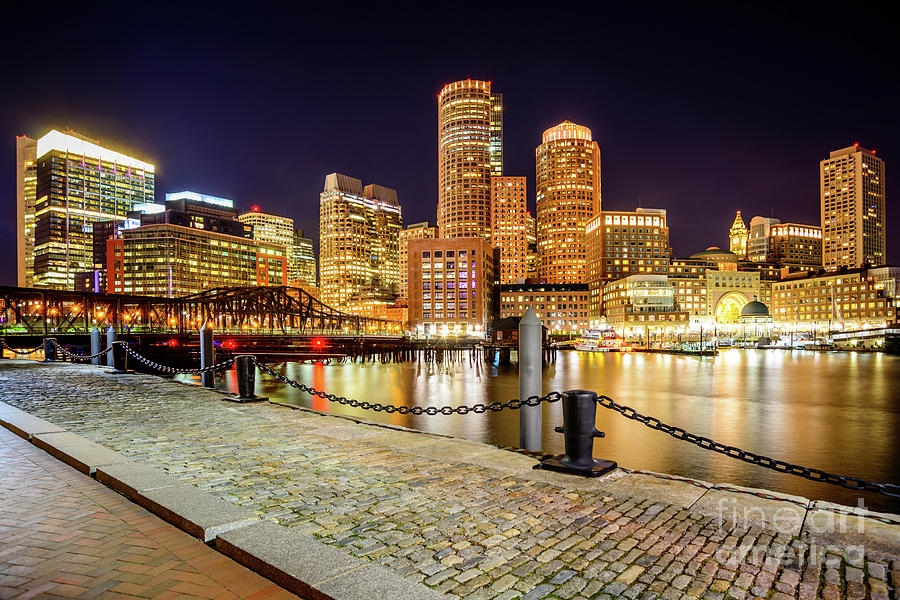
\includegraphics[height=\paperheight]{boston-skyline}
};

\begin{scope}
\clip(current page.north east) -- (current page.north west) --
 ([yshift=-1cm]current page.west) --([yshift=-3.3cm]current page.east) --cycle;
\node[at={([yshift=-1cm]current page.center)},anchor=south]{%
	
\includegraphics[height=5.8cm,trim=0cm 2.4cm 0cm 1.4cm,page=\value{page}]{night}
};
\end{scope}
%\node[at={(current page.center)},anchor=south]{%
%	
\includegraphics[height=\paperheight,page=\value{page}]{night}
%};

% Image credit of background
\node[at=(current page.south),yshift=0.25cm,text width=\paperwidth,font=\tiny,align=center,white]{%
	\url{https://images.fineartamerica.com/images/artworkimages/mediumlarge/1/boston-skyline-at-night-and-harborwalk-picture-paul-velgos.jpg}
};
\end{tikzpicture}


\foreach\x in {1,2,...,25}{%
  \ifodd\x \renewcommand\openclose{close}\else\renewcommand\openclose{open}\fi
  \only<\x>{%
  \vspace*{2cm}
  \includegraphics[scale=0.8]{marmot-\openclose}
\includegraphics[scale=0.85,trim=0cm 0.75cm 0cm 0cm]{marmot-\openclose}
\includegraphics[scale=0.9,trim=0cm 1.5cm 0cm 0cm]{marmot-\openclose}
\includegraphics[scale=0.95,trim=0cm 2.25cm 0cm 0cm]{marmot-\openclose}}}


\end{frame}
\end{document}
\AddToHook{shipout/foreground}{%
 \put(0.8\paperwidth,-0.8\paperheight)
 { 
\begin{tikzpicture}
   \marmot;
   \ifodd\value{page}
    \fill[draw=brown!30!black,fill=brown,line width=0.4pt] (0.145,1.51) arc [start angle=-20, end angle=-160, radius=0.16] -- cycle;
   \fi
   \bobblehat{xkcdMauve}{xkcdBrickRed}
   \end{tikzpicture}}}

\AddToHook{shipout/foreground}{%
 \put(0.7\paperwidth,-0.9\paperheight)
  { 
\begin{tikzpicture}
   \sheep;
   \ifodd\value{page}
    \fill[draw=brown!30!black,fill=brown,line width=0.4pt] (0.16,1.43) arc [start angle=-30, end angle=-90, radius=0.16] -- (0,1.164) -- (0,1.3485) arc [start angle=-90, end angle=-150, radius=0.16]-- cycle;
   \fi
   \bobblehat{xkcdMauve}{xkcdBrickRed}
   \end{tikzpicture}
  }
  \put(0.6\paperwidth,-0.9\paperheight)
  {
\begin{tikzpicture}
   \hippo;
   \ifodd\value{page}
   \fill[draw=brown!30!black,fill=brown,line width=0.4pt] (0.125, 1.5) arc [start angle=-50, end angle=-130, radius=0.2] -- cycle;
   \fi
   \bobblehat{xkcdMauve}{xkcdBrickRed}
   \end{tikzpicture}
  }
  \put(0.5\paperwidth,-0.95\paperheight)
  {
\begin{tikzpicture}
   \bear;
   \ifodd\value{page}
   \fill[draw=brown!30!black,fill=brown,line width=0.4pt] (0.145, 1.38) arc [start angle=-20, end angle=-160, radius=0.16] -- cycle;\fi
   \begin{scope}%[scale=1.3,yshift=-4.2mm]
   \bobblehat{xkcdCloudyBlue}{xkcdDullBlue}
   \end{scope}
   \end{tikzpicture}}}



\begin{frame}
\vspace*{3cm}


\begin{tikzpicture}[scale=2]
\marmot;
\foreach\x in {1,2,...,10}{
  \ifodd\x \only<\x>{
 \fill[draw=brown!30!black,fill=brown,line width=0.4pt] (0.145,1.51) arc [start angle=-20, end angle=-160, radius=0.16] -- cycle;}\else\only<\x>{} \fi}
\bobblehat{xkcdAquamarine}{xkcdBlueGreen}
\end{tikzpicture}


\end{frame}
\end{document}
